\documentclass[a4paper,11pt,twoside]{article}
%\documentclass[a4paper,11pt,twoside,se]{article}

\usepackage{UmUStudentReport}
\usepackage{verbatim}   % Multi-line comments using \begin{comment}
\usepackage{courier}    % Nicer fonts are used. (not necessary)
\usepackage{pslatex}    % Also nicer fonts. (not necessary)
\usepackage[pdftex]{graphicx}   % allows including pdf figures
\usepackage{listings}
\usepackage{pgf-umlcd}
\usepackage{blindtext}
\usepackage{enumitem}
%\usepackage{lmodern}   % Optional fonts. (not necessary)
%\usepackage{tabularx}
%\usepackage{microtype} % Provides some typographic improvements over default settings
%\usepackage{placeins}  % For aligning images with \FloatBarrier
%\usepackage{booktabs}  % For nice-looking tables
%\usepackage{titlesec}  % More granular control of sections.

% DOCUMENT INFO
% =============
\department{Department of Computing Science}
\coursename{Application Development in Java 7.5 p}
\coursecode{5DV135}
\title{RadioInfo}
\author{Lorenz Gerber ({\tt{dv15lgr@cs.umu.se}} {\tt{lozger03@student.umu.se}})}
\date{2017-01-11}
%\revisiondate{2016-01-18}
\instructor{Johan Eliasson / Jan Erik Moström / Alexander Sutherland / Filip Allberg / Adam Dahlgren Lindström}


% DOCUMENT SETTINGS
% =================
\bibliographystyle{plain}
%\bibliographystyle{ieee}
\pagestyle{fancy}
\raggedbottom
\setcounter{secnumdepth}{2}
\setcounter{tocdepth}{2}
%\graphicspath{{images/}}   %Path for images

\usepackage{float}
\floatstyle{ruled}
\newfloat{listing}{thp}{lop}
\floatname{listing}{Listing}



% DEFINES
% =======
%\newcommand{\mycommand}{<latex code>}

% DOCUMENT
% ========
\begin{document}
\lstset{language=C}
\maketitle
\thispagestyle{empty}
\newpage
\tableofcontents
\thispagestyle{empty}
\newpage

\clearpage
\pagenumbering{arabic}

\section{Introduction}
The aim of this assignment was to develop an application that uses the open web API from `Sveriges Radio' (\textit{http://sverigesradio.se/api/documentation/v2/index.html}) to present the current radio program in a graphical user interface. 

\section{Usage} 

\subsection{Compiling from command line}
The source code for the Java application `RadioInfo' was divided into the packages `model', `view', `controller' and `data\_io'. The class containing the `main' method was contained in the base directory (default package). The following steps were conducted to build a jar application file:

\begin{verbatim}
mkdir build
javac -d ./build *java model/*.java view/*.java controller/*.java ./
model_io/*.java
cd build
jar cvfe RadioInfo.jar RadioInfoMain *.class model/ view/ controller/ ./
data_io/
\end{verbatim}

The `.jar' file is named `RadioInfo.jar' while the `main' containing class is name `RadioInfoMain'. The source code is provided in a separate tar.gz file. 



\subsection{Program Usage}
On some operating systems, double click on `RadioInfo.jar' will start the application. From the command line on OSX and -nix systems, it can be invoked by: \\
\\
\verb+java -jar RadioInfo.jar+ \\
\\
The application will start and directly show a three split window with the program table on the left, textual program description om the middle and program image on the right.
Radio programs that started before the current time are shown with white font on black background while programs to be broadcasted are shown with black font on white background.
To get more information about a specific program, the user can click in the table on a program. If available, the respective description and image will be shown in the middle and right side panel.
The `RadioInfo' application has a menu bar with two drop-down menus: File and Channels. In the file menu, `Reload' allows to refresh the program table by reloading it from the web, while `quit' will terminate the background update service and exit the application. In the `channels' menu, all available channels are shown and can be selected. After selection, the respective program is loaded from the net and visualized in the leftmost panel.
There is a background process running that will update the program table once every hour. 


\section{System Description}
The whole application is structured according to the \textit{Model-View-Controller} pattern. This was also followed for packaging the source files. Besides the `model', `view' and `controller' package, there is also a `data\_io' package that contains the XML classes for interacting with the web API. The `RadioInfoMain' class can be found in the base directory.
An UML diagram with all classes (figure \ref{fig:overview}) gives a good first overview of the program structure.

\begin{figure}[p]
  \centering
  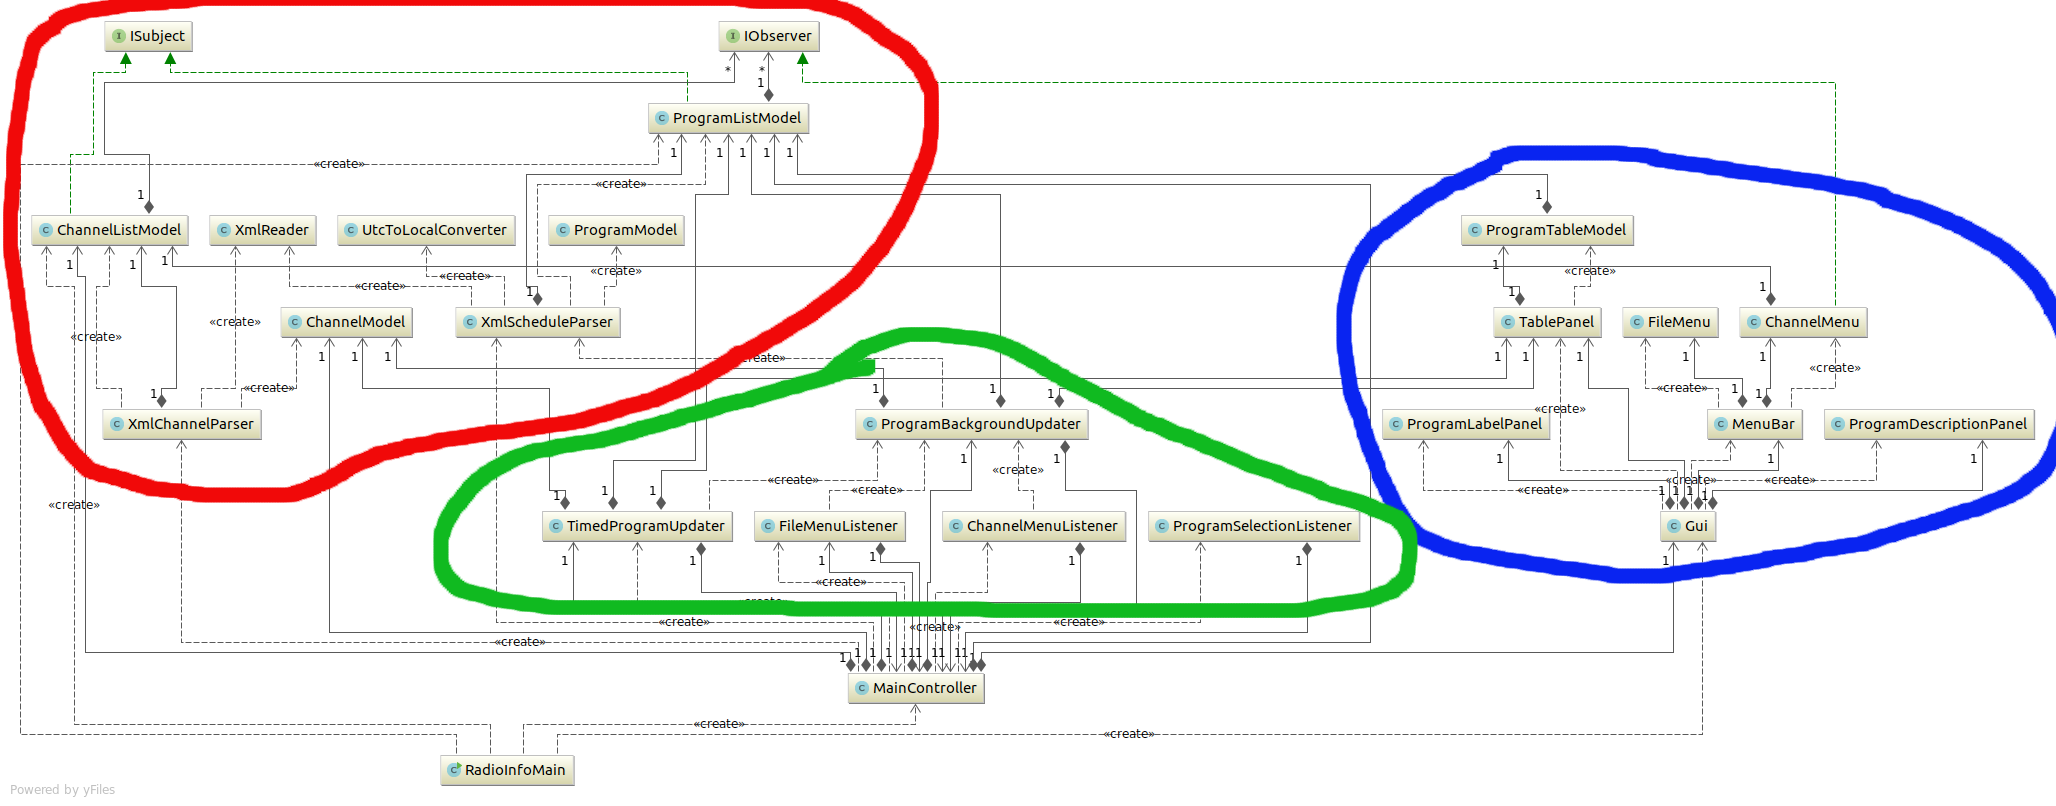
\includegraphics[width=1.5\textwidth, angle=90]{overview_color.png}
  \caption{This figure shows an overview of all classes. The red circle marks the model classes related to program logic. The blue circle marks the GUI classes and green marks the controllers.}
  \label{fig:overview}
\end{figure}

The whole GUI structure can be seen marked with blue. Within the red circle is the application logic. On the bottom, not marked with color, there are the classes RadioMainInfo and MainController. As the name says, RadioInfoMain contains the `main' method and initiates bootstrapping the whole application. The MainController is really the connection between program logic, GUI and also all the auxiliary controllers marked with green. A more detailed account for the different functional groups of the application follows below.


\subsection{Core Structure and Model-View-Controller separation}
In figure \ref{fig:basic}, the basic structure of the application is shown. The `main' method in \textit{RadioInfoMain Class} starts a new Swing thread, by defining an anonymous \textit{runnable} method. In this method first the main data containers `channels' (\textit{ChannelListModel Class}) and `programs' (\textit{ProgramListModel Class}) are set up. Next the GUI instance is started and used as method argument to the `main' (\textit{MainController}). `main' then bootstraps the whole application. 


\begin{figure}[p]
  \centering
  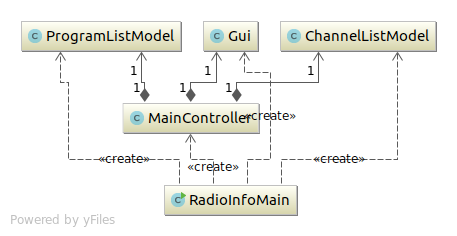
\includegraphics[width=0.8\textwidth]{basicUML.png}
  \caption{\textit{This figure shows the basic structure of the application: The main method is in the RadioInfoMain.class. It defines and starts a new thread. In this thread the two main data containers, channels (ChannelListModel class) and programs (ProgramListModel Class) are set up. Then it instantiates the GUI and the MainController. The main controller takes a reference to the GUI instance as construction argument. The main controller bootstraps the whole application then.}}
  \label{fig:basic}
  \end{figure}


\subsection{Data Models and Data Handling}
`radio channel' and `radio program' were chosen to represent the real-world objects modeled in the application. Each a class \textit{ChannelModel} and \textit{ProgramModel} was setup. These classes don't have much functionality besides the storage of information. Further, two container classes two hold an number of the aforementioned data models were constructed: \textit{ChannelListModel} and \textit{ProgramListModel}. Both classes extend the Java Collections \textit{ArrayList} and implement also the \textit{iterable} interface. As it can bee seen in figure \ref{fig:dataModels}, the `data\_io' classes \textit{XmlChannelParser} and \textit{XmlSchedulParser} can construct the respective data container classes. The XML parser classes make use of a general \textit{XmlReader} class that provides the DOM tree. 

\begin{figure}[p]
  \centering
  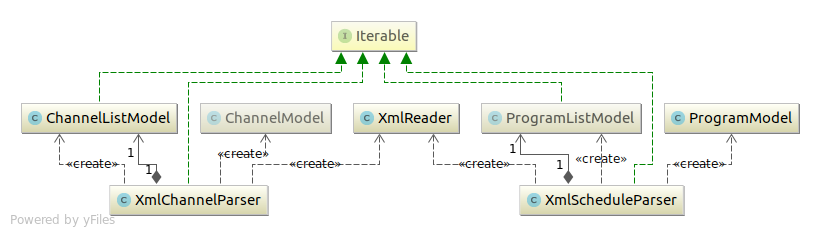
\includegraphics[width=1\textwidth]{dataModelsUML.png}
  \caption{\textit{This figure shows the data models used in RadioInfo Application. The real-world objects `radio channel' and `radio program' are represented by the classes \textit{ChannelModel} and \textit{ProgramModel}. They don't possess much functionality and are mostly used for storing and passing the information during run-time. Further, there exist two container class two agglomerate a number of channels or programs, \textit{ChannelListModel} and \textit{ProgramListModel}. They both make use of the XML classes to obtain the data.}}
  \label{fig:dataModels}
\end{figure}

\subsubsection{Parsing the Schedule Data}
The web API for reading the schedule data (e.g. \textit{api.sr.se/api/v2/scheduledepisodes?channelid=164}) has several filter options. However, there is no possibility to filter for a time range, as requested in the assignment specification (+/- 12 hours). Hence, after reading extra data from the web API it has to be filtered to the appropriate time range. The date/time information from the web API is in UTC and has to be converted to local time. For this a small helper class, \textit{UtcToLocalConverter} was implemented.
To keep the ProgramListModel class generic, it does not know about XML converters. Instead, it takes a iterator<ProgamModel> in the constructor to fill it's data structure. In fact, the XML parser uses internally also a `ProgramListModel' to store the `ProgramModel' objects. The XML parser class contains a helper function that constructs a LocalDateTime range from one day before today to one day after today. This date range in form of an ArrayList is then used to query the web API in sequence for the respective dates. The `ProgramListModel' class has methods implemented to filter the entries to the +/- 12 hours range.
The parser classes have multiple constructors to allow simplified unit testing without web access. The test directory contains a downloaded XML document from the web API to run test. The parser classes make use of the \textit{XmlReader} class which reads the XML document and puts the data into a DOM tree. It can handle both URLs to local files and web URLs.


\subsection{The Graphical User Interface}
The graphical user interface (GUI) is kept very simple and clean. It was chosen to implement a \textit{GridLayout} design using three JPanel derived classes in a row for representing the whole application. Channel selection and data refreshing/reload is obtained through a JMenuBar with two JMenu's.

\begin{figure}[p]
  \centering
  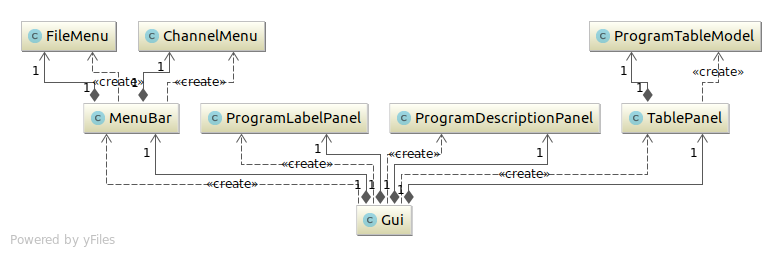
\includegraphics[width=1\textwidth]{guiUML.png}
  \caption{\textit{This figure shows the simple structure of the graphical user interface. TablePanel, ProgramDescriptionPanel and ProgramLablePanel are all sub-classed from JPanel. They are organized in a JFrame using a \textit{GridLayout} layout manager that specifies three columns and one row. The MenuBar (sub-classed from JMenuBar) has two sub menus (sub-classed from JMenu): FileMenu and ChannelMenu.}}
  \label{fig:gui}
\end{figure}

The main area for user interaction is the JTable which contains visualizes the program titles, start and end time. It was chosen to use \textit{AbstractTableModel} as base class and build an own table model implementation, \textit{ProgramTableModel}. Compared to the simpler alternative, using `DefaultTableModel' the current implementation allows to use directly a different data source for the table. This design decision was taken after reading the Oracle/Java tutorial on Tables \cite{javatables}.

\subsubsection{User Interactions and Action Events}
A set of `observable/observer' interfaces was used for both the ChannelListmodel and ProgramListModel as subjects and the `channelMenu' as `observable'. Otherwise, ActionEventListener derived classes were setup for `ChannelMenu', `FileMenu' and the table (`ProgramSelectionListener'). All action event listeners are setup from the main controller class.   



\subsection{Threads and Thread Safety}
The application uses separate threads for updating the data: SwingWorkers are invoked to not block the UI while pulling new data from the web API. As these operations could be potentially slow, they could be invoked again while the old one is still running. More over, user interactions such as clicking in the table potentially access the same data containers: `programs' and `channels' and `current channel'.
To make the application thread safe, synchronized methods where used. As all data-containers get accessed through the MainController, the getters and setters in the MainController for the respective data containers were synchronized. 


\subsection{Summary of Design Patterns}
The used design patterns were described throughout the text in their application context. Here follows a brief summary of the used patterns.
\begin{description}[align=left, labelwidth=4cm]
\item [Model-View-Controller] The whole application is built and structured according to this pattern.
\item [Observer-Observable] This pattern was implemented for the data containers to be observable and fire updates when they change. 
\item [Iterator] As Java implements iterator by default, it was easy to implement the interface iterable. This was done for ProgramListModel, mainly to be able to use it directly as a source for Java Streams. 
\item [Factory Method] This pattern was not implemented by the author, but used through the DocumentBuilderFactory class in Java. 
\end{description}


\section{Limitations}
Known limitations of the application are currently a rather sloppy implementation of the GUI. This is not functionally but it should be optimized for window re-sizing etc. Further, there has not been implemented a proper visualization of the LocalDateTime class in the table model. This results in the rather bulky original stringTo visualization.
The author started the project with good intentions using Test Driven Design. This can be seen in the XML parser classes. However, the TDD approach got lost when starting with a basic UI and was not taken up again for the Model classes. There should be implemented a number of unit tests for the model classes.  
Functionally, and specifically in terms of thread safety, the author was however not able to provoke uncontrolled application states during manual testing.

\addcontentsline{toc}{section}{\refname}
\bibliography{references}

\end{document}
